\documentclass[a4paper,12pt,french] {article}

\usepackage[sujet]{../../../Style}

\fancyhead[L]{02/02/2022}
\fancyhead[C]{\textbf{DS5 : Fonctions polynomiales de degré 2}}
\fancyhead[R]{\premiere ST2S 2}

\renewcommand{\baselinestretch}{1.2}

% Passage en A3
%\geometry{a3paper,landscape,bottom=7mm,twocolumn}
%\setlength{\headwidth}{39cm} %42cm-2*margin pour fancyhdr


\begin{document}

\rem{L'usage de la calculatrice est autorisé. La propreté et l'orthographe seront prises en compte. Tout le devoir peut être fait sur le sujet.}

Nom: \hfill Prénom: \hfill \

\begin{exercice} \

\compo[0.7]
{
On se donne la parabole $\mathscr P$ ci-contre, et $f:x \mapsto ax^2+c$ la fonction de degré deux associée.
\begin{enumerate}
\item Quel est le signe de $a$? \dotfill
\item Donner la valeur de $c$: \dotfill
\item Placer le sommet de $\mathscr P$ et préciser ses coordonnées: \dotfill
\item Quel est l'axe de symétrie de $\mathcal P$? \dotfill
\item Donner les deux racines de $f$: \dotfill
\item En utilisant le point $A(1;-3)$, déterminer $a$, et en déduire l'équation de $\mathscr P$, sous forme développée puis factorisée.
\end{enumerate}
}
{
\begin{centrer}
\begin{tikzpicture}
\begin{axis}[
styleglobal,
width=0.9*\linewidth,
xmin=-4, xmax=4,
ymin=-5, ymax=5,
xtick distance=1,
ytick distance=1,
]
\addplot[styleplot,domain=(-4:4)]{(x^2-4} node[pos=0.7,below right]{$\mathscr P$};;
\end{axis}
\end{tikzpicture}
\end{centrer}
}

\points 5
\end{exercice}

\begin{exercice}
Une micro-entreprise fabrique des ventilateurs. On note $B(x)$ le résultat financier (bénéfice ou perte), exprimé en centaines d'euros, réalisé par l'entreprise pour la production de $x$ centaines de ventilateurs, lorsque $x \in [0;+\infty[$. On a $B(x)=-2x^2+90x-400$.
\begin{enumerate}
\item Calculer $B(30)$ et interpréter ce résultat dans le contexte de l'exercice.

\points 3

\item On admet que, pour tout $x$ de l'intervalle  $[2;+\infty[$, on a $f(x)=-2(x-5)(x-40)$.\\
Dresser le tableau de signes de la fonction $B$ sur l'intervalle $[0;+\infty[$:
\compo[0.4]
{
\points 6
}
{
\begin{center}
\begin{tikzpicture}
\tkzTabInit[lgt=2.5]{ /1, /4}{0,,$+\infty$}
\end{tikzpicture}
\end{center}
}
\item A quels volumes de production de ventilateurs le résultat réalisé par
l'entreprise est-il positif ?

\points 3

\item Déterminer la valeur du bénéfice maximal et le volume de production correspondant.

\points 3

\end{enumerate}
\end{exercice}

\begin{exercice} \

\begin{enumerate}
\item En justifiant, relier chacune des paraboles $\mathscr P_1$, $\mathscr P_2$ et $\mathscr P_3$ aux fonctions ci-dessous:

\compo[0.4]
{
\begin{itemize}[leftmargin=20pt]
\item $f:x \mapsto -2x^2+2$
\item $g:x \mapsto (x-1)(x+3)$
\item $h:x \mapsto 5(x-0.5)(x+0.5)$

\points {10}

\end{itemize}
}
{
\begin{centrer}
\begin{tikzpicture}
\begin{axis}[
styleglobal,
width=0.9*\linewidth,
xmin=-4, xmax=4,
ymin=-5, ymax=5,
xtick distance=1,
ytick distance=1,
]
\addplot[styleplot]{((x-1)*(x+3)} node[pos=0.65,above right]{$\mathscr P_1$};
\addplot[styleplot,color=blue,densely dashed]{-2*x^2+2} node[pos=0.65,above right]{$\mathscr P_2$};
\addplot[styleplot,color=red,densely dotted]{5*(x-0.5)*(x+0.5)} node[pos=0.65,above right]{$\mathscr P_3$};
\end{axis}
\end{tikzpicture}
\end{centrer}
}

\item On considère la fonction $i:x \mapsto y=-0.5(x+4)(x-1)$. Tracer la parabole associée à la fonction $i$ sur le repère ci-dessous. Si besoin, on pourra noter des calculs ci-dessous.

\points 4

\begin{centrer}
\begin{tikzpicture}
\begin{axis}[
styleglobal,
width=0.9*\linewidth,
xmin=-6, xmax=6,
ymin=-4, ymax=4,
xtick distance=1,
ytick distance=1,
]
%\addplot[styleplot]{-0.5*(x+4)*(x-1)};
\end{axis}
\end{tikzpicture}
\end{centrer}

\item Dresser le tableau de variations de $i$. Justifier.

\compo[0.5]
{
\points 5
}
{
\begin{center}
\begin{tikzpicture}
\tkzTabInit[lgt=1.2]{ /1, /3}{$- \infty$,,$+ \infty$}
\end{tikzpicture}
\end{center}
}

\end{enumerate}
\end{exercice}

\begin{exercice} \

\compo[0.5]
{
\strut Après l'administration d'un antibiotique, la population d'une bactérie, exprimée en dizaine de milliers, en fonction du temps (en heures), est modélisée par la fonction $f$ sur l'intervalle $[0;3]$ représentée ci-contre.

On administre l'antibiotique à l'instant $t=0$.
}
{
\begin{centrer}
\begin{tikzpicture}
\begin{axis}[
styleglobal,
hauteurproptick,
width=0.9*\linewidth,
xmin=-0.5, xmax=4,
ymin=-0.5, ymax=4.5,
xtick distance=1,
ytick distance=1,
%ylabel style={sloped like y axis,anchor=north east},
%ylabel style={at={(ticklabel cs:1)},anchor=near ticklabel opposite,rotate=90},
ylabel={Population (\times 10000)},
xlabel={Temps (h)},
%xlabel near ticks,
%ylabel near ticks,
%xlabel shift={5mm},
%major grid style={line width=1pt},
]
\addplot[styleplot,domain=(0:3)]{-0.8*x^2+1.2*x+3.6} node[pos=0.8,above right] {$\mathscr C_f$};
%\node[stylepoint,inner sep=1pt,fill=blue,label={-60:A}] (A) at (5.3,2.9) {};
%\node[stylepoint,inner sep=1pt,fill=blue,label={60:B}] (B) at (5.3,3.5) {};
%\node[stylepoint,inner sep=1pt,fill=blue,label={-60:J}] (J) at (0,2) {};
%\draw[very thick] (A) -- (B);
\end{axis}
\end{tikzpicture}
\end{centrer}
}
\newpage
\begin{enumerate}
\item \textbf{Étude graphique}:\\
En exploitant la figure, répondre aux questions suivantes:
\begin{enumerate}
\item Quel est le nombre de bactéries à l'instant où l'on administre l'antibiotique?

\points 2

\item Quel est le nombre de bactéries lorsque $t = 0,5$ h ?

\points 2

\item Quel semble être la population maximale de bactéries?

\points 2

\end{enumerate}
      \item \textbf{Étude de la fonction $f$:}\\
      La fonction $f$ est définie sur l'intervalle $[0; 3]$ par $f(t)=-0,8t^2+1,2t+3,6$:
      
\begin{enumerate}
\item Calculer $f(0)$ et $f(1.5)$. Interpréter ces résultats par une phrase.

\points 4

\item En utilisant la symétrie de la courbe $C_f$, calculer la population maximale de bactéries.

\points 4
      
 \end{enumerate}     

\item Montrer que $f(t)=-0.8(t-3)(t+1,5)$, pour $t \in [0;3]$.

\points 4

\end{enumerate}

\end{exercice}

\end{document}